\documentclass[tikz]{standalone}
\usepackage{tikz}
\usetikzlibrary{calc}
\usetikzlibrary{arrows}
\begin{document}
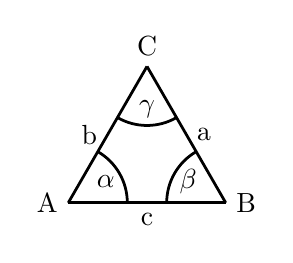
\begin{tikzpicture}[]
\coordinate (A) at (0,0);
\coordinate (B) at (2,0);
\coordinate (C) at (60:2);
\def\bogenR{0.75}
\def\winkelPos{0.55}
\draw[line width=1pt] node[left]{A} (A) --node[below]{c} (B) node[right]{B} ;
\draw[line width=1pt] (A) --node[left]{b}  (C) node[above]{C} ;
\draw[line width=1pt] (B) --  node[right]{a}   (C) ;
\draw [line width=1pt] ($(A) + (\bogenR,0)$) arc (0:60:\bogenR);
\draw [line width=1pt] ($(B) + (180:\bogenR)$) arc (180:120:\bogenR);
\draw [line width=1pt] ($(C) + (240:\bogenR)$) arc (240:300:\bogenR);
\node at (30:\winkelPos) {$\alpha$};	
\node  at ($(B)+(150:\winkelPos)$) {$\beta$};
\node  at ($(C)+(270:\winkelPos)$) {$\gamma$};
\end{tikzpicture}

\end{document}
